\section{State machine}
    \begin{minipage}[t]{0.48\columnwidth}
        \vspace{0pt} % <-- ensures top alignment
        Le \textbf{Finite State Machine} (FSM) sono macchine a base di circuiti logici sequenzali.\\
        Sono in grado quindi 
        di eseguire operazioni logiche e di poterle memorizzare in modo da consegnare in uscita una funzione
        che non solo è dipendente dagli Input attuali ma anche (o solo) dallo stato attuale (memorizzato con gli input precedenti).\\
        Le tre alternative proposte di seguito sono delle possibilità di incapsulamento standardizzato
        della funzione desiderata, qualunque essa sia.\\
        - Cit. Alessio Ciceri
    \end{minipage}
    \hfill
    \begin{minipage}[t]{0.48\columnwidth}
        \vspace{0pt} % <-- ensures top alignment
        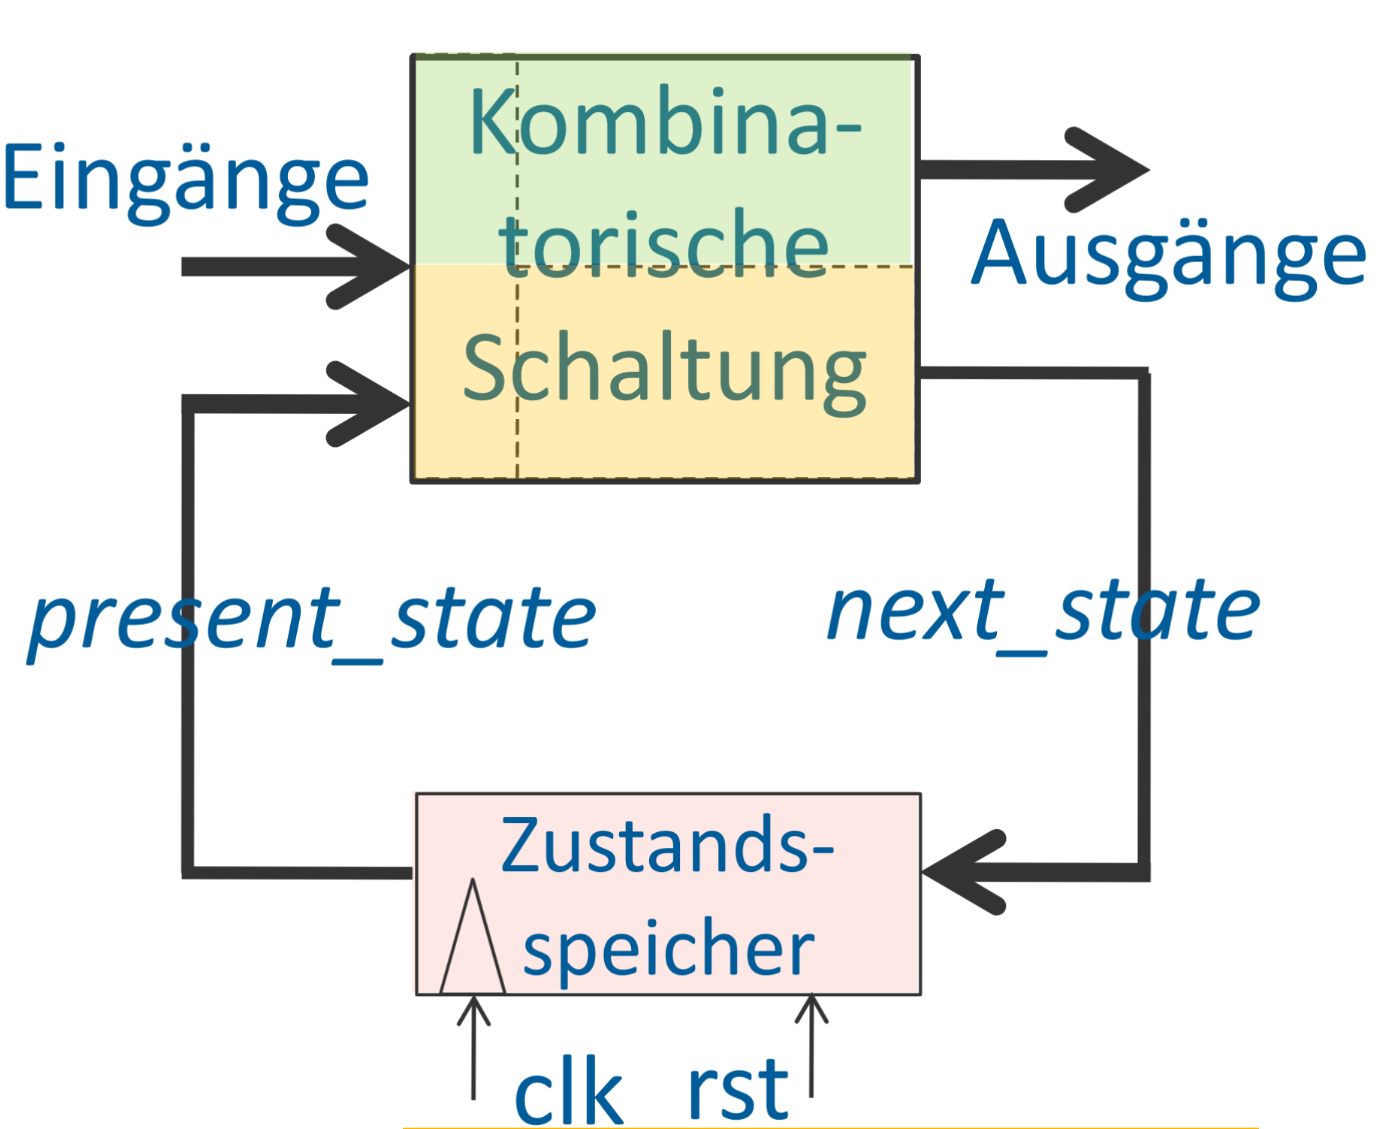
\includegraphics[width=\linewidth]{Images/FSMGeneralizzata.png}
    \end{minipage}%
    

% ==================================== FAMIGLIE FSM ====================================
    %---------- MEDWEJDJEW ----------
    \subsection{Medwedjew}
    \begin{minipage}[t]{0.48\columnwidth}
        \vspace{0pt} % <-- ensures top alignment
        Composta da una un blocco di logica combinatoria(G) che risolve la funzione desiderata e da un blocco di memoria(Z)
        che memorizza gli stati.\\ 
        => Gli Input e lo stato attuale della FSM vengono processati da una logica combinatoria(G)\\
        => Il risultato della logica viene memorizzato nella Zustandspeicher(Z)\\
        => L'uscita è esattamente la copia di tutti gli stati memorizzati(s).
    \end{minipage}%
    \hfill
    \begin{minipage}[t]{0.48\columnwidth}
        \vspace{0pt} % <-- ensures top alignment
        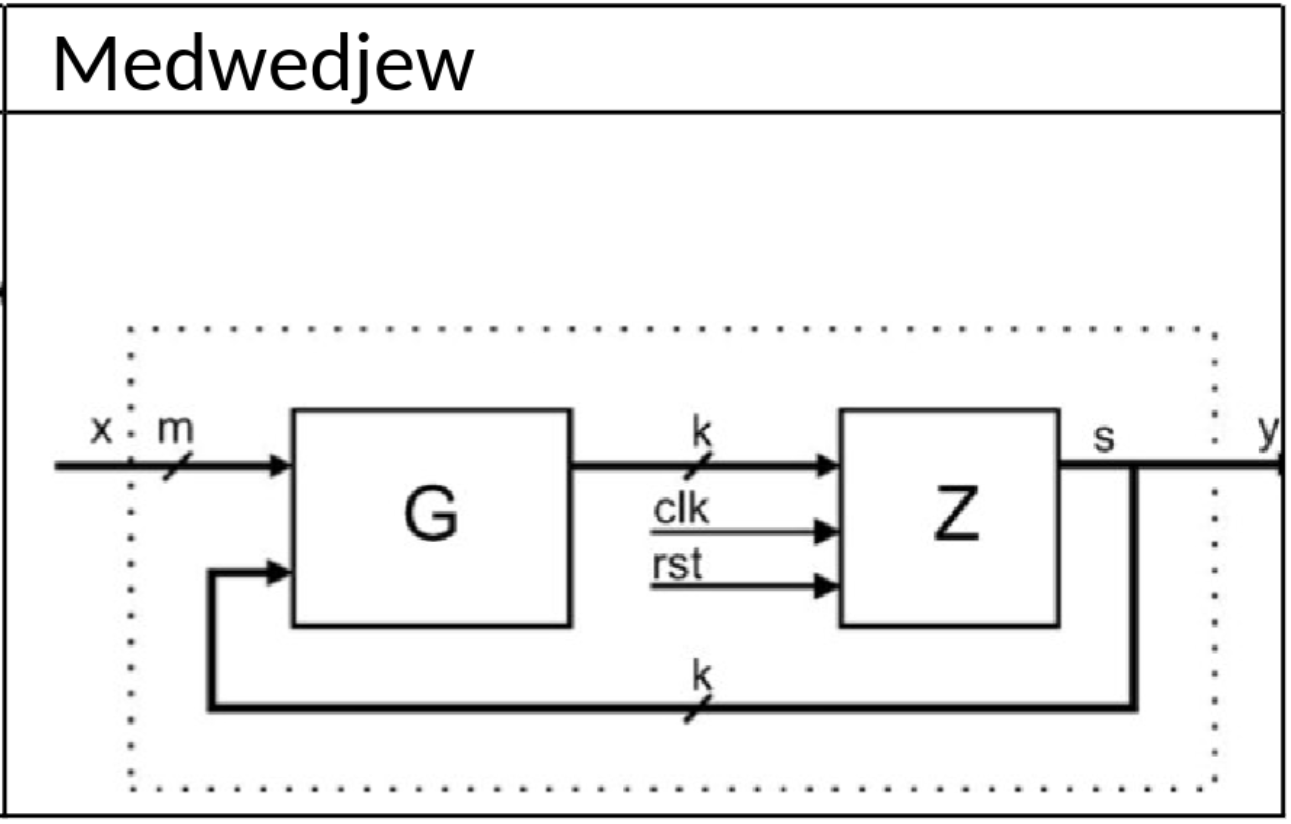
\includegraphics[width=\linewidth]{Images/Medwedjew.png}
    \end{minipage}

    %---------- MOORE ----------
    \subsection{Moore}
    \begin{minipage}[t]{0.48\columnwidth}
        \vspace{0pt} % <-- ensures top alignment
        Come Medwedjew ma con una logica dedicata sul ramo di output(s).\\
        Tipicamente utile per output più complessi/numerosi rispetto agli stati memorizzati(k $\neq$ n).\\
        => logica combinatoria aggiuntiva sul ramo d'uscita (F)\\
        => Più efficiente di Medwedjew per la memorizzazione degli stati
    \end{minipage}%
    \hfill
    \begin{minipage}[t]{0.48\columnwidth}
        \vspace{0pt} % <-- ensures top alignment
        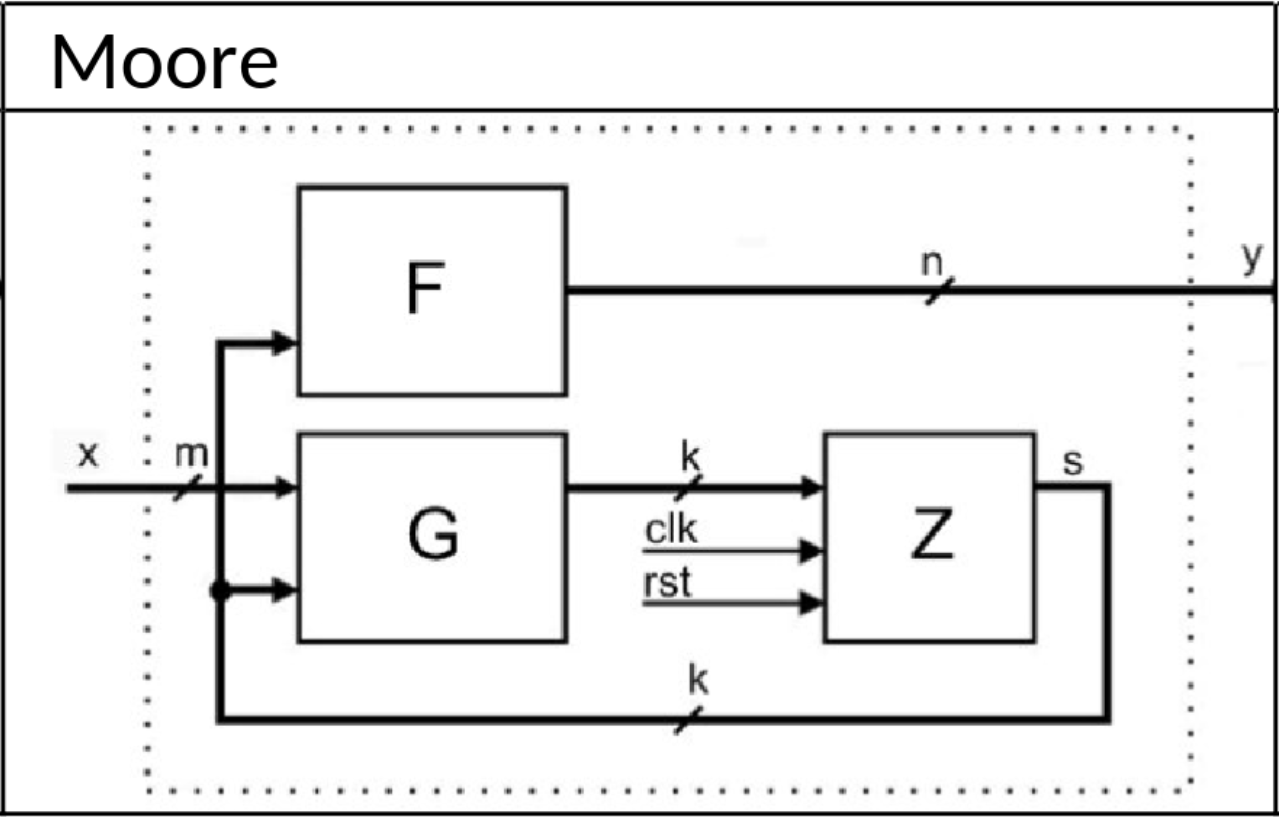
\includegraphics[width=\linewidth]{Images/Moore.png}
    \end{minipage}

    %---------- MEALY ----------
    \subsection{Mealy}
    \begin{minipage}[t]{0.48\columnwidth}
        \vspace{0pt} % <-- ensures top alignment
        Si tratta della Versione Moore dove la logica sul ramo d'uscita è dipendente anche a segnali provenienti direttamente
        dagli input della FSM\\
        => Necessaria se y dipende asincronamente da delle entrate\\
        => Più complessa, spesso riducibile a Moore
    \end{minipage}%
    \hfill
    \begin{minipage}[t]{0.48\columnwidth}
        \vspace{0pt} % <-- ensures top alignment
        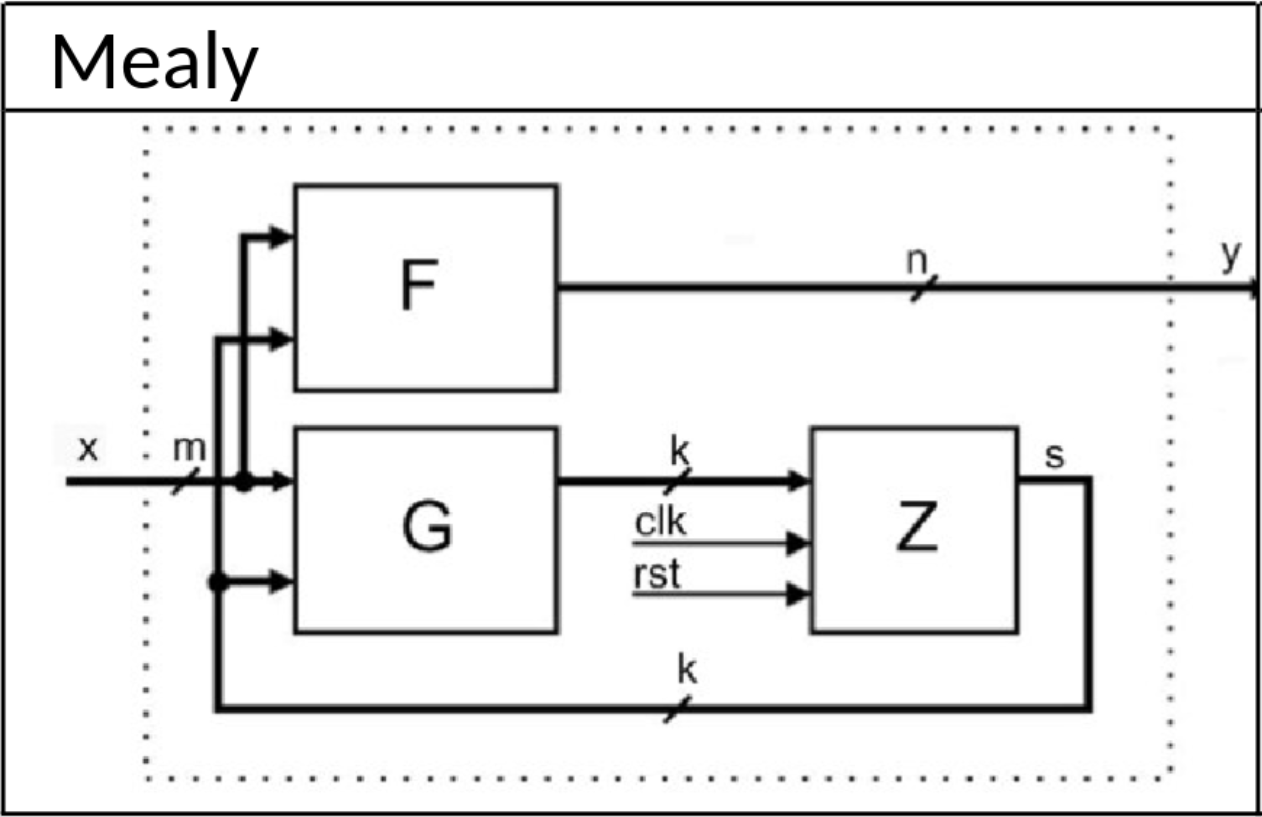
\includegraphics[width=\linewidth]{Images/Mealy.png}
    \end{minipage}


% ==================================== CODICE SCHELETRO FSM ====================================
    \subsection{Codice scheletro FSM (G,Z,F)}
        \begin{lstlisting}[language=VHDL, escapeinside={(*@}{@*)}]

            G: process(present_state, inputs)
            begin
                next_state <= de fault_state;
                    case present_state is
                        when X_state =>
                            next_state <= Y_state;
                        when others =>
                            next_state <= R_state;
                end case;
            end process;

            Z: process(clk)
            begin
                if clk(*@'@*)event and clk = '1' then
                    if reset = '1' then
                        present_state <= reset_state;
                    else
                        present_state <= next_state;
                    end if;
                end if;
            end process;

            F: process(present_state, …)
            begin
                oup <= default_value;
                case present_state is
                    when X_state =>
                        oup <= "1001";
                    when others =>
                        oup <= "1111";
                end case;
            end process;

        \end{lstlisting}


% ==================================== CODIFICA DEGLI STATI ====================================
    \subsection{Codifica degli stati}
    Gli stati di una FSM possono essere codificati in diversi modi, tra cui:
    \begin{itemize}
        \item \textbf{Codifica binaria}: ogni stato è rappresentato da un codice binario unico.
        \item \textbf{Codifica Gray}: simile alla codifica binaria, ma le transizioni tra stati adiacenti cambiano solo un bit alla volta.
        \item \textbf{Codifica one-hot}: ogni stato è rappresentato da un bit attivo, con tutti gli altri bit a zero.
        \item \textbf{Codifica one-cold}: simile alla codifica one-hot, ma solo un bit è a zero e tutti gli altri sono attivi.
    \end{itemize}